% =====================================================================
%  Guía de repaso: métricas y estrategias de variación de hiperparámetros
%  Documento auxiliar de la Tarea Académica 1 - Deep Learning para Finanzas
%  Compilar con pdflatex (dos pasadas). Figuras en ./figuras/
% =====================================================================
\documentclass[11pt,a4paper]{article}

\usepackage[utf8]{inputenc}
\usepackage[T1]{fontenc}
\usepackage[spanish,es-noshorthands,es-tabla]{babel}
\usepackage{mathptmx}
\usepackage{courier}
\usepackage{microtype}
\usepackage{amsmath,amssymb}
\usepackage[margin=2.3cm]{geometry}
\usepackage{setspace}
\setstretch{1.2}
\setlength{\parindent}{0pt}
\setlength{\parskip}{6pt}

\usepackage{graphicx}
\graphicspath{{figuras/}}
\usepackage{booktabs,tabularx,array,float}
\usepackage[labelfont=bf,textfont=it,labelsep=period,skip=4pt,font=small]{caption}
\usepackage{xcolor}
\definecolor{azul}{HTML}{1C5CAB}
\definecolor{azulclaro}{HTML}{EAF2FC}
\definecolor{naranja}{HTML}{B4501F}
\definecolor{naranjaclaro}{HTML}{FDF0E8}
\definecolor{gris}{HTML}{F4F4F2}

\usepackage[most]{tcolorbox}
\newtcolorbox{ejemplo}[1][]{enhanced,breakable,colback=azulclaro,colframe=azul,boxrule=0.5pt,
  arc=2pt,left=6pt,right=6pt,top=4pt,bottom=4pt,fonttitle=\bfseries\small,
  title={Ejemplo#1}}
\newtcolorbox{clave}{enhanced,breakable,colback=naranjaclaro,colframe=naranja,boxrule=0.5pt,
  arc=2pt,left=6pt,right=6pt,top=4pt,bottom=4pt,fonttitle=\bfseries\small,title={Idea clave}}
\newtcolorbox{proyecto}{enhanced,breakable,colback=gris,colframe=gray!60,boxrule=0.5pt,
  arc=2pt,left=6pt,right=6pt,top=4pt,bottom=4pt,fonttitle=\bfseries\small,title={En nuestro proyecto}}

\usepackage{titlesec}
\titleformat{\section}{\normalfont\Large\bfseries\color{azul}}{\thesection}{0.6em}{}[\vspace{-6pt}\color{azul}\rule{\linewidth}{0.6pt}]
\titleformat{\subsection}{\normalfont\large\bfseries}{\thesubsection}{0.5em}{}
\titleformat{\subsubsection}{\normalfont\normalsize\bfseries\itshape}{}{0em}{}
\titlespacing*{\section}{0pt}{16pt}{8pt}
\titlespacing*{\subsection}{0pt}{12pt}{3pt}

\usepackage{fancyhdr}
\pagestyle{fancy}
\fancyhf{}
\fancyhead[L]{\small\scshape Guía de repaso — métricas e hiperparámetros}
\fancyhead[R]{\small\thepage}
\renewcommand{\headrulewidth}{0.3pt}

\usepackage{needspace}
\usepackage{enumitem}
\setlist{itemsep=2pt,topsep=2pt}
\usepackage[hidelinks]{hyperref}
\newcommand{\code}[1]{\texttt{#1}}

\begin{document}

% ------------------------------ Portada ------------------------------
\begin{titlepage}
\centering
{\large\scshape Pontificia Universidad Católica del Perú\par}
\vspace{0.2cm}
{\normalsize Deep Learning para Finanzas (1FIN58)\par}
\vspace{3.5cm}
{\color{azul}\rule{\linewidth}{1pt}}\par\vspace{0.6cm}
{\Huge\bfseries\color{azul} Guía de repaso\par}
\vspace{0.4cm}
{\LARGE Métricas de clasificación y estrategias\\[0.1cm] de variación de hiperparámetros\par}
\vspace{0.5cm}{\color{azul}\rule{\linewidth}{1pt}}\par
\vspace{1cm}
{\large Documento auxiliar de la Tarea Académica 1\\ Predicción de impago en préstamos de Lending Club\par}
\vfill
{\large Sebastián Estefano Hernández Muñaqui\par}
\vspace{0.8cm}
{\normalsize Lima, octubre de 2026\par}
\end{titlepage}

\tableofcontents
\newpage

% =====================================================================
\section*{Cómo usar esta guía}
\addcontentsline{toc}{section}{Cómo usar esta guía}

Esta guía reúne, de forma teórica, todos los conceptos que se usaron en el informe final: la preparación de los datos, las métricas, la política de umbral, el tratamiento del desbalance, las estrategias de búsqueda de hiperparámetros, cada hiperparámetro de la red, los modelos base y las técnicas de interpretabilidad. Cada concepto tiene tres capas:

\begin{itemize}
\item \textbf{Teoría}: la definición y, cuando aplica, la fórmula.
\item \textbf{Ejemplo}: un cálculo pequeño, hecho a mano, en un recuadro azul.
\item \textbf{En nuestro proyecto}: cómo apareció el concepto en la tarea, con los números reales de la corrida, en un recuadro gris.
\end{itemize}

Los recuadros naranjas («Idea clave») resumen lo que conviene recordar. Al final hay una tabla resumen de hiperparámetros (Sección~\ref{sec:resumen}) y preguntas de repaso con sus respuestas (Sección~\ref{sec:preguntas}).

Notación: $y\in\{0,1\}$ es la etiqueta real (1 = impago), $\hat p\in[0,1]$ la probabilidad de impago que da el modelo, $t$ el umbral de decisión y $\hat y = \mathbb{1}[\hat p \ge t]$ la predicción.

% =====================================================================
\needspace{8\baselineskip}
\section{Preparación de los datos}

\subsection{Entrenamiento, validación y prueba}

Los datos se dividen en tres conjuntos con funciones distintas:

\begin{itemize}
\item \textbf{Entrenamiento}: el modelo ajusta sus pesos con estos datos.
\item \textbf{Validación}: se usa para \emph{tomar decisiones}: elegir hiperparámetros, el umbral y el modelo final, y decidir cuándo detener el entrenamiento.
\item \textbf{Prueba}: se consulta \emph{una sola vez}, al final, para estimar el desempeño con datos nunca usados en ninguna decisión.
\end{itemize}

La partición es \textbf{estratificada} cuando cada conjunto conserva la proporción de clases de la base completa, algo importante cuando una clase es rara.

\begin{proyecto}
Se separó 20\,\% para prueba y luego 20\,\% del resto para validación: $0.8\times0.8=0.64$, es decir, 64\,\% de entrenamiento (12\,739 préstamos), $0.8\times0.2=0.16$, es decir, 16\,\% de validación (3\,185) y 20\,\% de prueba (3\,981). Los tres conjuntos tienen 14.8\,\% de impagos.
\end{proyecto}

\subsection{Fuga de información}

Hay \textbf{fuga de información} (\textit{data leakage}) cuando algún dato de validación o prueba influye en el entrenamiento. Un caso típico: calcular la mediana para imputar, o el mínimo y el máximo para escalar, usando toda la base. Así, el modelo «ve» indirectamente datos que luego se usan para evaluarlo, y las métricas resultan optimistas.

\begin{clave}
Todo lo que se \emph{aprende} de los datos (medianas, modas, mínimos, máximos, categorías) se ajusta \textbf{solo con entrenamiento} (\code{fit}) y luego se \textbf{aplica} a validación y prueba (\code{transform}).
\end{clave}

\subsection{Imputación y codificación \textit{one-hot}}

La \textbf{imputación} rellena valores faltantes: con la mediana en las variables numéricas (robusta a valores extremos) y con la moda en las categóricas. La \textbf{codificación \textit{one-hot}} convierte una variable categórica con $k$ categorías en $k$ columnas binarias.

\begin{ejemplo}[: one-hot]
La variable \code{home\_ownership} con valores \{RENT, OWN, MORTGAGE\} se convierte en tres columnas. Un préstamo con valor OWN queda como $(\text{RENT},\text{OWN},\text{MORTGAGE}) = (0,1,0)$.
\end{ejemplo}

\subsection{Escalado MinMax}

El escalado MinMax lleva cada variable numérica al intervalo $[0,1]$:
\begin{equation}
x' = \frac{x - x_{\min}}{x_{\max} - x_{\min}},
\end{equation}
donde $x_{\min}$ y $x_{\max}$ se calculan en entrenamiento. Si un dato de prueba supera esos extremos, queda fuera de $[0,1]$, y eso es correcto: no se reajusta el escalador.

\begin{ejemplo}[: MinMax (valores ilustrativos)]
Si en entrenamiento la tasa de interés va de 5\,\% a 25\,\%, un préstamo al 18.3\,\% queda en $x'=(18.3-5)/(25-5)=0.665$. El ingreso anual, de 4\,000 a 6\,000\,000, se lleva a la misma escala $[0,1]$. Sin escalar, el ingreso dominaría los productos $w\cdot x$ solo por su magnitud.
\end{ejemplo}

\begin{proyecto}
En el avance inicial, el MinMaxScaler se construía antes de que existiera la matriz de variables y su salida nunca llegaba a los modelos: las redes se entrenaban sin escalar. La corrección fue un único \code{ColumnTransformer} ajustado solo con entrenamiento. Resultaron 49 variables: 12 numéricas y 37 indicadoras.
\end{proyecto}

% =====================================================================
\needspace{8\baselineskip}
\section{Métricas de evaluación}\label{sec:metricas}

\subsection{Matriz de confusión}

Con un umbral $t$, cada predicción cae en una de cuatro casillas:

\begin{table}[H]
\centering
\begin{tabular}{lcc}
\toprule
 & Predicho 0 (pagado) & Predicho 1 (impago) \\
\midrule
Real 0 (pagado) & VN (verdadero negativo) & FP (falso positivo) \\
Real 1 (impago) & FN (falso negativo) & VP (verdadero positivo) \\
\bottomrule
\end{tabular}
\end{table}

En crédito, un \textbf{FN} es aprobar un préstamo que no se pagará (pérdida de capital) y un \textbf{FP} es rechazar o encarecer a un buen cliente (pérdida de negocio).

\subsection{Exactitud, precisión, \textit{recall} y F1}

\begin{align}
\text{Exactitud} &= \frac{VP+VN}{VP+VN+FP+FN} \\
\text{Precisión} &= \frac{VP}{VP+FP} \qquad \text{(de los que marqué como impago, ¿cuántos lo eran?)} \\
\text{Recall} &= \frac{VP}{VP+FN} \qquad \text{(de los impagos reales, ¿cuántos detecté?)} \\
F_1 &= \frac{2\cdot \text{Precisión}\cdot\text{Recall}}{\text{Precisión}+\text{Recall}}
\end{align}

El F1 es la media armónica de la precisión y el \textit{recall}: solo es alto si ambas lo son. La \textbf{exactitud balanceada} promedia el \textit{recall} de cada clase:
\begin{equation}
\text{Exactitud balanceada} = \tfrac12\left(\frac{VP}{VP+FN} + \frac{VN}{VN+FP}\right).
\end{equation}

\begin{ejemplo}[: la red mejorada en prueba, umbral de validación 0.178]
La matriz es VN = 2\,522, FP = 870, FN = 293, VP = 296 (3\,981 préstamos, 589 impagos).
\begin{itemize}
\item Exactitud $=(296+2522)/3981 = 0.708$.
\item Precisión $=296/(296+870)=0.254$.
\item \textit{Recall} $=296/(296+293)=0.503$.
\item F1 $=2(0.254)(0.503)/(0.254+0.503)=0.337$.
\item Exactitud balanceada $=\tfrac12(0.503 + 2522/3392) = \tfrac12(0.503+0.744)=0.623$.
\end{itemize}
\end{ejemplo}

\begin{clave}
Con desbalance, la exactitud engaña. Si el 85.2\,\% de los préstamos se paga, el modelo que siempre dice «pagado» tiene una exactitud de 85.2\,\% y un F1 de 0. Por eso se priorizan F1, AP y AUC.
\end{clave}

\subsection{Pérdida logarítmica (\textit{log-loss})}

Es la función que minimiza la red (entropía cruzada binaria):
\begin{equation}
\mathcal{L} = -\frac1N\sum_{i=1}^{N}\Big[y_i\ln \hat p_i + (1-y_i)\ln(1-\hat p_i)\Big].
\end{equation}
Castiga con fuerza las predicciones seguras y equivocadas. A diferencia del F1, no depende del umbral, sino de qué tan bien \emph{calibradas} están las probabilidades.

\begin{ejemplo}[: log-loss]
\textbf{Un préstamo.} Si $\hat p=0.342$ y el préstamo era impago, su pérdida es $-\ln 0.342 = 1.07$; si se pagó, es $-\ln 0.658 = 0.42$.

\textbf{Predictor constante.} Un modelo que asigna a todos la prevalencia $\hat p=0.148$ tiene
$\mathcal{L}= -[0.148\ln0.148+0.852\ln0.852] = 0.283+0.137 = 0.419$.
\end{ejemplo}

\begin{proyecto}
La red de 100 capas terminó con una pérdida de 0.419, justo la del predictor constante: había colapsado a predecir la prevalencia para todos (AUC 0.57). Las redes útiles bajaron a $\approx 0.39$.
\end{proyecto}

\subsection{Curva ROC, AUC y Gini}

La curva ROC grafica el \textit{recall} (tasa de verdaderos positivos) frente a la tasa de falsos positivos $FP/(FP+VN)$ al recorrer todos los umbrales. El \textbf{AUC} es el área bajo esa curva y tiene una interpretación probabilística:
\begin{equation}
\text{AUC} = P\big(\hat p(\text{impago}) > \hat p(\text{pagado})\big),
\end{equation}
es decir, la probabilidad de que un impago elegido al azar reciba un puntaje mayor que un pagado elegido al azar. Vale 0.5 para un modelo aleatorio y 1 para uno perfecto. El \textbf{índice de Gini}, muy usado en riesgo de crédito, es una reescala:
\begin{equation}
\text{Gini} = 2\,\text{AUC} - 1 \in [-1, 1].
\end{equation}

\subsection{Curva precisión--\textit{recall} y precisión promedio (AP)}

La curva PR grafica la precisión frente al \textit{recall}. La \textbf{precisión promedio} la resume:
\begin{equation}
\text{AP} = \sum_n (R_n - R_{n-1})\,P_n .
\end{equation}
Su línea base no es 0.5, sino la \textbf{prevalencia} de la clase positiva. Con clases desbalanceadas es más exigente que el AUC, porque mide qué tan «limpios» son los primeros préstamos marcados como riesgosos (Saito \& Rehmsmeier, 2015).

\begin{ejemplo}[: AUC y AP a mano]
Cinco préstamos ordenados de mayor a menor puntaje, con etiquetas reales $(1,0,1,0,0)$: hay 2 impagos y 3 pagados.

\textbf{AUC}: hay $2\times3=6$ pares (impago, pagado). El impago del puesto 1 supera a los 3 pagados; el del puesto 3 supera a 2 (los de los puestos 4 y 5). AUC $=5/6=0.833$.

\textbf{AP}: se recorre la lista y se mira cada vez que aparece un impago.
En el puesto 1, $P=1/1$ y $R=1/2$; en el puesto 3, $P=2/3$ y $R=2/2$.
AP $=(0.5-0)\cdot 1 + (1-0.5)\cdot\tfrac23 = 0.5+0.333 = 0.833$.

\textbf{Gini} $=2(0.833)-1=0.667$.
\end{ejemplo}

\begin{figure}[H]
\centering
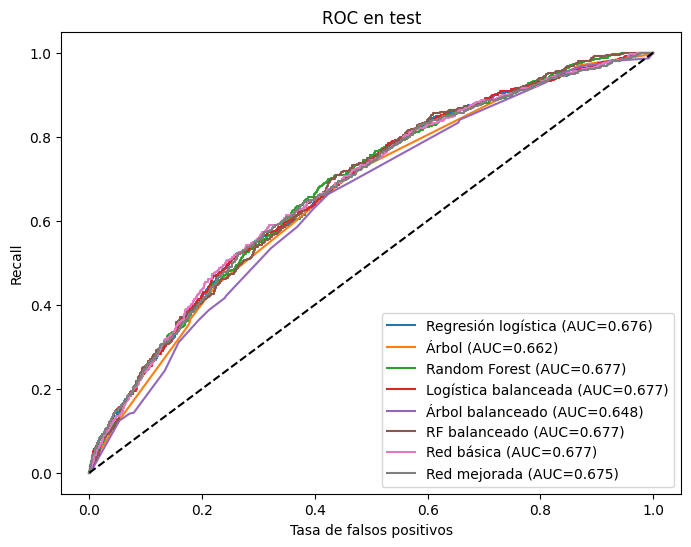
\includegraphics[width=0.48\linewidth]{c38_2.png}\hfill
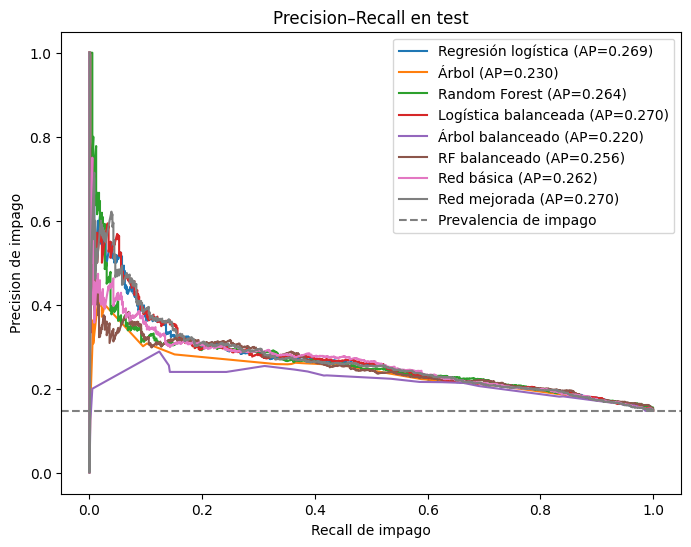
\includegraphics[width=0.48\linewidth]{c38_3.png}
\caption{Curvas ROC (izquierda) y precisión--\textit{recall} (derecha) de los ocho modelos en el conjunto de prueba del proyecto. La línea discontinua horizontal de la derecha es la prevalencia (0.148), que es el AP de un modelo aleatorio.}
\end{figure}

\subsection{\texorpdfstring{$R^2$}{R2} sobre probabilidades}

Es el coeficiente de determinación calculado entre $y$ y $\hat p$: $R^2=1-\sum(y-\hat p)^2/\sum(y-\bar y)^2$. Es una métrica descriptiva, no de clasificación: vale 0 para el predictor constante y puede ser negativa si las probabilidades están desplazadas.

\begin{proyecto}
La red básica con pesos balanceados tuvo $R^2=-0.70$, aunque su AUC era casi igual al de la versión sin pesos (0.684 frente a 0.686). Los pesos empujan todas las probabilidades hacia arriba: el orden de los préstamos no cambia, pero los valores quedan lejos de 0 y 1.
\end{proyecto}

\subsection{¿Qué métrica depende de qué?}

\begin{table}[H]
\centering
\small
\begin{tabularx}{\linewidth}{lccX}
\toprule
Métrica & ¿Depende del umbral? & Línea base aleatoria & Qué mide \\
\midrule
Exactitud & sí & prevalencia de la clase mayoritaria (0.852) & aciertos totales \\
Precisión / \textit{recall} / F1 & sí & -- & desempeño en la clase impago \\
Exactitud balanceada & sí & 0.5 & promedio del \textit{recall} de ambas clases \\
\textit{Log-loss} & no & 0.419 (constante) & calibración de probabilidades \\
AUC / Gini & no & 0.5 / 0 & capacidad de ordenar (ranking) \\
AP & no & 0.148 (prevalencia) & ranking enfocado en la clase rara \\
\bottomrule
\end{tabularx}
\caption{Resumen de métricas. Las líneas base corresponden a la prevalencia del proyecto.}
\end{table}

% =====================================================================
\needspace{8\baselineskip}
\section{El umbral de decisión}

La red entrega una probabilidad; el umbral $t$ la convierte en decisión. El valor $t=0.5$ no tiene nada de especial: con una clase rara, las probabilidades de casi todos los préstamos quedan por debajo de 0.5 y el modelo nunca marca impagos.

Bajar el umbral aumenta el \textit{recall} y reduce la precisión. Un criterio común es elegir el $t$ que \textbf{maximiza el F1 en validación}, congelarlo y aplicarlo sin cambios a prueba (Figura~\ref{fig:umbral}).

\begin{figure}[H]
\centering
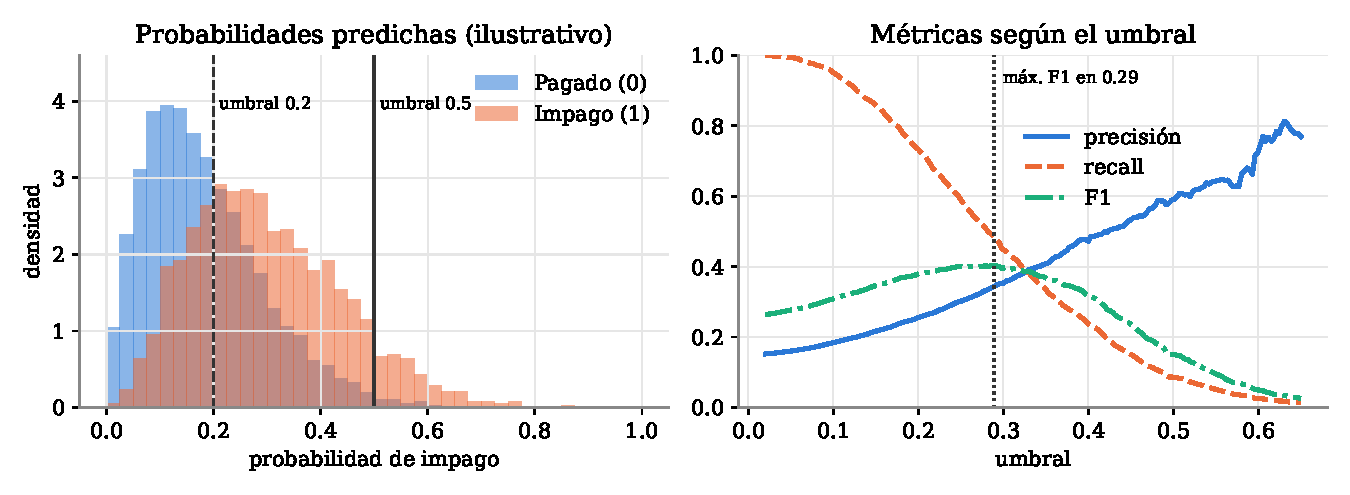
\includegraphics[width=\linewidth]{umbral.pdf}
\caption{Ejemplo ilustrativo con datos simulados. Izquierda: las probabilidades de ambas clases se superponen y casi todas quedan bajo 0.5. Derecha: al subir el umbral, el \textit{recall} cae y la precisión sube; el F1 alcanza su máximo en un umbral bajo.}\label{fig:umbral}
\end{figure}

\begin{clave}
Cambiar el umbral \textbf{no cambia} el AUC ni el AP, porque no altera el orden de las probabilidades. Solo decide cuántos préstamos se marcan como impago.
\end{clave}

\begin{proyecto}
La red mejorada tiene F1 = 0 con $t=0.5$, porque su probabilidad máxima en toda la prueba es 0.342. Con el umbral de validación $t=0.178$, su F1 en prueba es 0.337.
\end{proyecto}

% =====================================================================
\needspace{8\baselineskip}
\section{Desbalance de clases y \texttt{class\_weight}}

Con pesos de clase, la pérdida de cada observación se multiplica por el peso de su clase. Con la opción \code{'balanced'} de scikit-learn:
\begin{equation}
w_c = \frac{N}{K\cdot N_c},
\end{equation}
donde $N$ es el total, $K=2$ el número de clases y $N_c$ el número de observaciones de la clase $c$.

\begin{ejemplo}[: pesos del proyecto]
En entrenamiento, $N=12\,739$, con $N_1=1\,883$ impagos y $N_0=10\,856$ pagados.
$w_1 = 12\,739/(2\cdot1\,883)=3.383$ y $w_0=12\,739/(2\cdot10\,856)=0.587$. Equivocarse con un impago «cuesta» $3.383/0.587\approx5.8$ veces más.
\end{ejemplo}

\subsection{Pesos y umbral son casi equivalentes}

Ponderar las clases desplaza las probabilidades. En la escala de \textit{log-odds}, el desplazamiento es aproximadamente $\ln(w_1/w_0)$, lo mismo que mover el umbral.

\begin{ejemplo}[: de un umbral a otro]
La logística sin pesos tiene umbral óptimo 0.185, es decir, $\text{logit}(0.185)=\ln(0.185/0.815)=-1.483$. Sumando $\ln(3.383/0.587)=1.752$ se obtiene 0.269, que equivale a una probabilidad de $1/(1+e^{-0.269})=0.567$. El umbral óptimo de la logística \emph{balanceada} fue 0.564: prácticamente el mismo clasificador.
\end{ejemplo}

\begin{proyecto}
Con pesos, el F1 con umbral 0.5 de la red básica subió de 0.004 a 0.355, pero el AP casi no cambió (0.2640 frente a 0.2638). Como la selección se hacía por AP, se conservó la versión sin pesos, y el desbalance se resolvió con el umbral.
\end{proyecto}

% =====================================================================
\needspace{8\baselineskip}
\section{Estrategias de búsqueda de hiperparámetros}

Los \textbf{parámetros} (pesos y sesgos) se aprenden con el gradiente. Los \textbf{hiperparámetros} (capas, neuronas, tasa de aprendizaje, etc.) se fijan antes de entrenar y se eligen comparando el desempeño en validación.

\subsection{Búsqueda en malla (\textit{grid search})}

Prueba todas las combinaciones de una lista de valores. Es exhaustiva, pero el número de entrenamientos crece de forma multiplicativa.

\begin{ejemplo}[: costo de una malla completa]
Con los valores del proyecto (2 de balanceo, 4 optimizadores, 3 tasas, 3 lotes, 4 activaciones, 5 profundidades, 5 anchos, 4 formas, 2 de \textit{dropout}, 3 de regularización, 5 de parada y 3 de épocas) habría
$2\cdot4\cdot3\cdot3\cdot4\cdot5\cdot5\cdot4\cdot2\cdot3\cdot5\cdot3 = 2\,592\,000$ combinaciones. A 100\,s por entrenamiento serían unos 8 años de cómputo.
\end{ejemplo}

\subsection{Búsqueda aleatoria (\textit{random search})}

Sortea combinaciones al azar dentro de rangos. Con el mismo presupuesto suele rendir mejor que la malla, porque casi siempre solo unos pocos hiperparámetros importan de verdad y el muestreo aleatorio prueba más valores distintos de cada uno (Bergstra \& Bengio, 2012).

\subsection{Búsqueda secuencial (descenso por coordenadas)}

Varía \textbf{un hiperparámetro por etapa}, elige el mejor y lo deja fijo para las etapas siguientes. El costo es la \emph{suma} de los valores probados, no el producto.

\textbf{Ventajas:} es barata y fácil de interpretar, porque cada etapa aísla un efecto.

\textbf{Desventajas:}
\begin{itemize}
\item Ignora interacciones. La mejor tasa de aprendizaje para una red de 1 capa puede no serlo para una de 20.
\item El resultado depende del \textbf{orden} de las etapas.
\item Si una etapa no incluye el valor vigente como candidato, se ve obligada a cambiar aunque empeore.
\end{itemize}

\subsection{Búsqueda iterativa desde una referencia}

Cada hiperparámetro se varía \emph{por separado} partiendo siempre de la misma configuración de referencia, y luego se combinan los ganadores. Mide efectos individuales sin arrastre, pero los óptimos individuales no tienen por qué sumarse: al combinarlos, el resultado puede empeorar.

\begin{proyecto}
Se usó la búsqueda secuencial con 43 entrenamientos (unos 73 minutos). El orden fue: balanceo $\rightarrow$ optimizador $\rightarrow$ tasa de aprendizaje $\rightarrow$ lote $\rightarrow$ activación $\rightarrow$ capas $\rightarrow$ neuronas $\rightarrow$ distribución $\rightarrow$ \textit{dropout} $\rightarrow$ regularización $\rightarrow$ \textit{early stopping} $\rightarrow$ épocas. Primero se fija la optimización sobre una red pequeña y rápida, luego la arquitectura y al final el control del sobreajuste. En la etapa de \textit{dropout} no se incluyó el valor 0, y el AP bajó de 0.2721 a 0.2520.
\end{proyecto}

\subsection{Criterio de selección y semillas}

En cada etapa se elige por una métrica de validación. En el proyecto fue el AP, con el F1 de umbral optimizado y el AUC como desempates. Dos cuidados:
\begin{itemize}
\item \textbf{Una sola semilla} introduce ruido: diferencias de AP de 0.001--0.005 pueden deberse solo a la inicialización aleatoria. Repetir con varias semillas o con validación cruzada da más certeza.
\item \textbf{Reutilizar validación} en muchas decisiones la vuelve optimista. Por eso la prueba se reserva para el final.
\end{itemize}

% =====================================================================
\needspace{8\baselineskip}
\section{Hiperparámetros de optimización}

\subsection{Descenso por gradiente y sus variantes}

El entrenamiento actualiza los pesos en dirección contraria al gradiente de la pérdida:
\begin{equation}
w \leftarrow w - \eta\,\nabla_w \mathcal{L}.
\end{equation}
Según cuántos datos se usen para estimar el gradiente, se habla de descenso por lotes completos (toda la base), estocástico (un dato) o por \textbf{mini-lotes} ($B$ datos), que es lo habitual.

\subsection{Optimizadores}

\subsubsection{SGD}
Aplica directamente $w \leftarrow w - \eta g$, donde $g$ es el gradiente del mini-lote. Es simple, pero lento en valles alargados y sensible a la tasa $\eta$.

\subsubsection{SGD con momento}
Acumula una «velocidad» que promedia los gradientes recientes:
\begin{equation}
v \leftarrow \beta v + g, \qquad w \leftarrow w - \eta v, \qquad \beta=0.9 .
\end{equation}
Si el gradiente es constante, el paso efectivo tiende a $\eta/(1-\beta)=10\eta$: acelera en direcciones consistentes y amortigua las oscilaciones.

\subsubsection{RMSprop}
Divide el paso por la magnitud reciente del gradiente de cada peso:
\begin{equation}
s \leftarrow \rho s + (1-\rho)g^2, \qquad w \leftarrow w - \eta\,\frac{g}{\sqrt{s}+\varepsilon}.
\end{equation}
Los pesos con gradientes grandes dan pasos más cortos y los de gradientes pequeños, pasos más largos: es una tasa de aprendizaje adaptativa por peso.

\subsubsection{Adam}
Combina el momento (primer momento $m$) con RMSprop (segundo momento $v$) y corrige el sesgo inicial (Kingma \& Ba, 2015):
\begin{align}
m &\leftarrow \beta_1 m + (1-\beta_1) g, & v &\leftarrow \beta_2 v + (1-\beta_2) g^2,\\
\hat m &= \frac{m}{1-\beta_1^{\,k}}, & \hat v &= \frac{v}{1-\beta_2^{\,k}}, \qquad
w \leftarrow w - \eta\,\frac{\hat m}{\sqrt{\hat v}+\varepsilon},
\end{align}
con $\beta_1=0.9$, $\beta_2=0.999$ y $k$ el número de paso.

\begin{ejemplo}[: primer paso de Adam]
Con $g=0.2$ y $\eta=0.001$ en el paso $k=1$: $m=0.1\cdot0.2=0.02$ y $v=0.001\cdot0.04=0.00004$. Corrigiendo el sesgo, $\hat m=0.02/0.1=0.2$ y $\hat v=0.00004/0.001=0.04$. El paso es $0.001\cdot0.2/\sqrt{0.04}=0.001$.
Si el gradiente fuera $g=20$, el paso seguiría siendo $\approx0.001$: en Adam, el tamaño del paso lo controla $\eta$, no la escala del gradiente.
\end{ejemplo}

\begin{proyecto}
Con $\eta=0.001$ para todos, Adam ganó (AP 0.2661), seguido de Momentum (0.2646) y RMSprop (0.2643). SGD quedó atrás (0.2366) y no se estabilizó en 100 épocas. Esa tasa es pequeña para SGD, que suele necesitar alrededor de 0.01, así que la comparación favorece a los métodos adaptativos.
\end{proyecto}

\subsection{Tasa de aprendizaje \texorpdfstring{$\eta$}{eta}}

Es el hiperparámetro más influyente en el entrenamiento. Si es muy pequeña, el avance es lento; si es adecuada, la pérdida baja rápido y de forma estable; si es muy grande, los pasos saltan sobre el mínimo, oscilan o divergen (Figura~\ref{fig:lr}).

\begin{figure}[H]
\centering
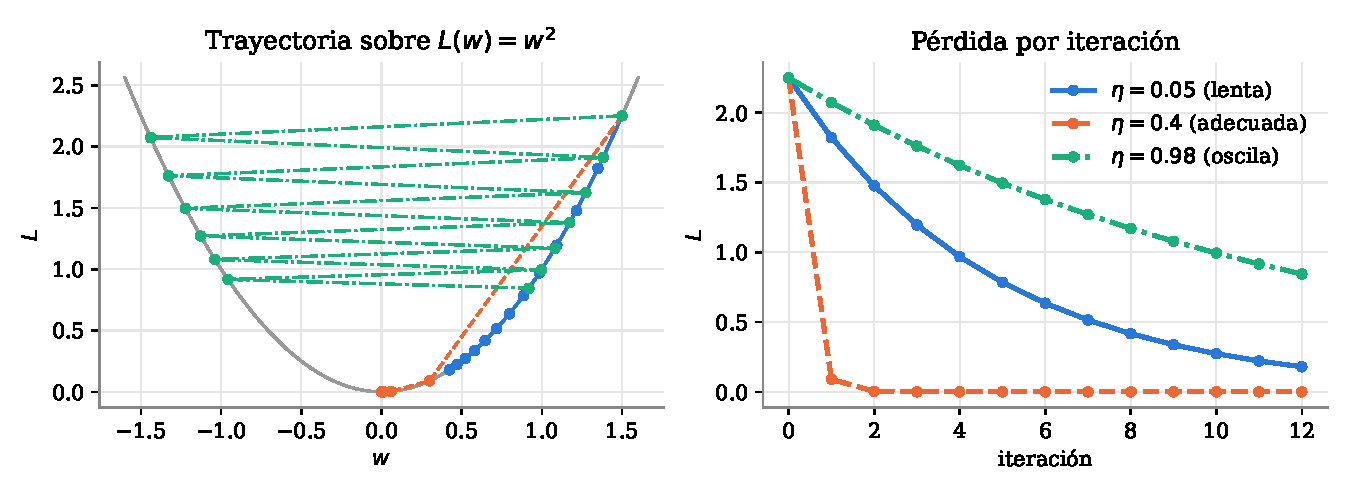
\includegraphics[width=\linewidth]{learning_rate.pdf}
\caption{Descenso por gradiente sobre $L(w)=w^2$ desde $w_0=1.5$. La actualización es $w\leftarrow(1-2\eta)w$: con $\eta=0.05$ avanza poco; con $\eta=0.4$ converge en pocos pasos; con $\eta=0.98$ el factor es $-0.96$ y el peso salta de un lado al otro del mínimo. Con $\eta>1$ divergería.}\label{fig:lr}
\end{figure}

\begin{proyecto}
Con Adam, $\eta=0.0001$ ganó (AP 0.2690). Con $\eta=0.01$ el entrenamiento se detuvo en 9 épocas, señal de pasos demasiado grandes.
\end{proyecto}

\subsection{Tamaño de lote \texorpdfstring{$B$}{B}}

Es el número de observaciones usadas para estimar cada gradiente. Un lote pequeño da gradientes más ruidosos pero más actualizaciones por época, y ese ruido a veces ayuda a generalizar. Un lote grande da gradientes más estables y aprovecha mejor la GPU, pero hace menos actualizaciones.

\begin{ejemplo}[: actualizaciones por época]
Con 12\,739 préstamos de entrenamiento: $B=32$ da $\lceil12739/32\rceil=399$ actualizaciones por época, $B=64$ da 200 y $B=128$ da 100.
\end{ejemplo}

\subsection{Épocas}

Una \textbf{época} es una pasada completa por el entrenamiento. Pocas épocas producen subajuste; demasiadas, sin control, producen sobreajuste. El número adecuado se decide mejor con \textit{early stopping} (Sección~\ref{sec:es}) que fijándolo a mano.

% =====================================================================
\needspace{8\baselineskip}
\section{Hiperparámetros de arquitectura}

\subsection{La neurona y la capa densa}

Una capa densa calcula $\mathbf{h} = g(W\mathbf{x}+\mathbf{b})$, donde $W$ es la matriz de pesos, $\mathbf{b}$ el sesgo y $g$ la función de activación. Una capa de $n_{\text{in}}$ entradas y $n_{\text{out}}$ neuronas tiene $n_{\text{in}}\,n_{\text{out}} + n_{\text{out}}$ parámetros.

\begin{ejemplo}[: conteo de parámetros]
\textbf{Red básica} (49 entradas, 1 capa de 100 neuronas, salida de 1 neurona):
$49\cdot100+100=5\,000$ en la capa oculta y $100+1=101$ en la salida, total $5\,101$.

\textbf{Red mejorada} (20 capas de 64): la primera tiene $49\cdot64+64=3\,200$; las otras 19 tienen $64\cdot64+64=4\,160$ cada una ($79\,040$ en total); la salida tiene $65$. Total: $82\,305$.
\end{ejemplo}

\subsection{Funciones de activación}

Sin activación no lineal, apilar capas equivale a una sola transformación lineal. Las activaciones comparadas en el proyecto fueron:
\begin{align*}
\text{ReLU: } & g(z)=\max(0,z) & \text{tanh: } & g(z)=\frac{e^z-e^{-z}}{e^z+e^{-z}}\\
\text{sigmoide: } & g(z)=\frac{1}{1+e^{-z}} & \text{ELU: } & g(z)=\begin{cases} z & z>0\\ e^{z}-1 & z\le0\end{cases}
\end{align*}

\begin{figure}[H]
\centering
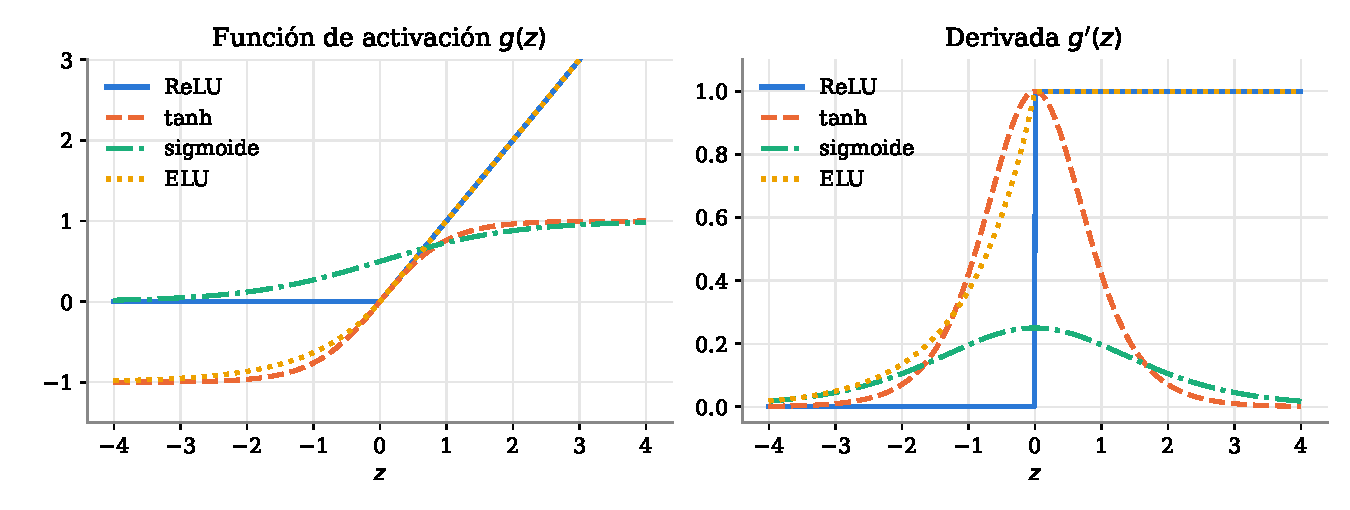
\includegraphics[width=\linewidth]{activaciones.pdf}
\caption{Activaciones (izquierda) y sus derivadas (derecha). La derivada de la sigmoide nunca supera 0.25 y la de tanh se anula en los extremos (saturación); la de ReLU vale 0 para $z<0$ («neuronas muertas»), y ELU mantiene un gradiente pequeño en esa zona.}
\end{figure}

\begin{table}[H]
\centering
\small
\begin{tabularx}{\linewidth}{lllX}
\toprule
Activación & Rango & Derivada máx. & Comentario \\
\midrule
ReLU & $[0,\infty)$ & 1 & barata, no satura para $z>0$; puede «morir» si $z<0$ siempre \\
tanh & $(-1,1)$ & 1 & centrada en cero; satura en los extremos \\
sigmoide & $(0,1)$ & 0.25 & se usa en la \emph{salida} para dar una probabilidad; en capas ocultas favorece el desvanecimiento del gradiente \\
ELU & $(-1,\infty)$ & 1 & como ReLU, pero suave y con salida negativa; evita neuronas muertas \\
\bottomrule
\end{tabularx}
\caption{Comparación de las activaciones.}
\end{table}

\begin{proyecto}
Con 1 capa, tanh ganó (AP 0.2765, el mejor de toda la búsqueda), con ELU muy cerca (0.2757). La salida fue siempre una sigmoide, para obtener una probabilidad de impago.
\end{proyecto}

\subsection{Profundidad y desvanecimiento del gradiente}

Por la regla de la cadena, el gradiente que llega a la primera capa es un producto de derivadas de todas las capas siguientes. Si esas derivadas son menores que 1, el producto se desvanece exponencialmente con la profundidad (Glorot \& Bengio, 2010).

\begin{ejemplo}[: desvanecimiento]
Con sigmoide, cada derivada es como máximo 0.25. Tras 20 capas el factor es a lo sumo $0.25^{20}\approx 9\times10^{-13}$: las primeras capas prácticamente no aprenden.
\end{ejemplo}

\begin{figure}[H]
\centering
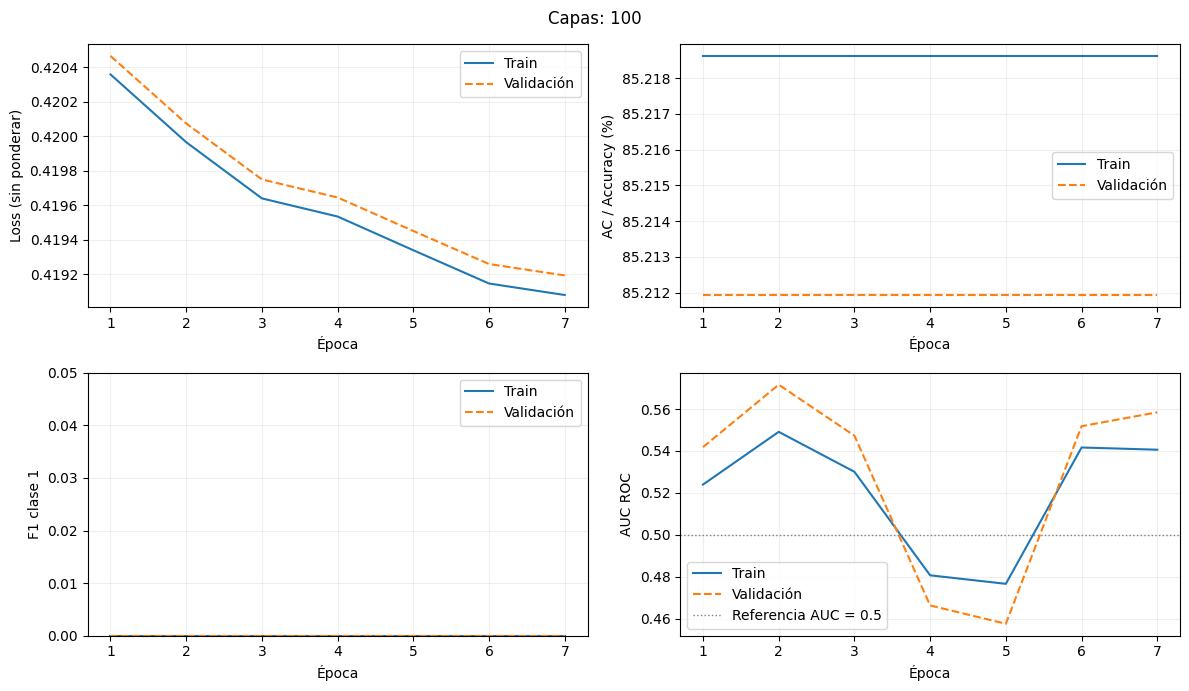
\includegraphics[width=0.75\linewidth]{c20_4.png}
\caption{La red de 100 capas del proyecto: la pérdida casi no cambia (cuarta cifra decimal) y el AUC oscila alrededor de 0.5.}
\end{figure}

\subsection{Ancho (neuronas por capa)}

Más neuronas dan más capacidad de representación, pero también más parámetros, más riesgo de sobreajuste y más costo. En el proyecto, con 20 capas, ganaron 64 neuronas; de 128 a 512 la red dejó de marcar impagos.

\subsection{Distribución de neuronas entre capas}

Con el mismo número de capas y el mismo total de neuronas, el reparto puede tener distintas formas (Figura~\ref{fig:formas}):
\begin{itemize}
\item \textbf{Uniforme}: todas las capas iguales.
\item \textbf{Creciente}: pocas neuronas al inicio y más al final.
\item \textbf{Embudo (decreciente)}: comprime la información de forma progresiva hacia la salida. Es la forma más usada en clasificación.
\item \textbf{Cuello de botella}: comprime hasta el centro y luego expande. Es la idea del \textit{autoencoder}.
\end{itemize}

\begin{figure}[H]
\centering
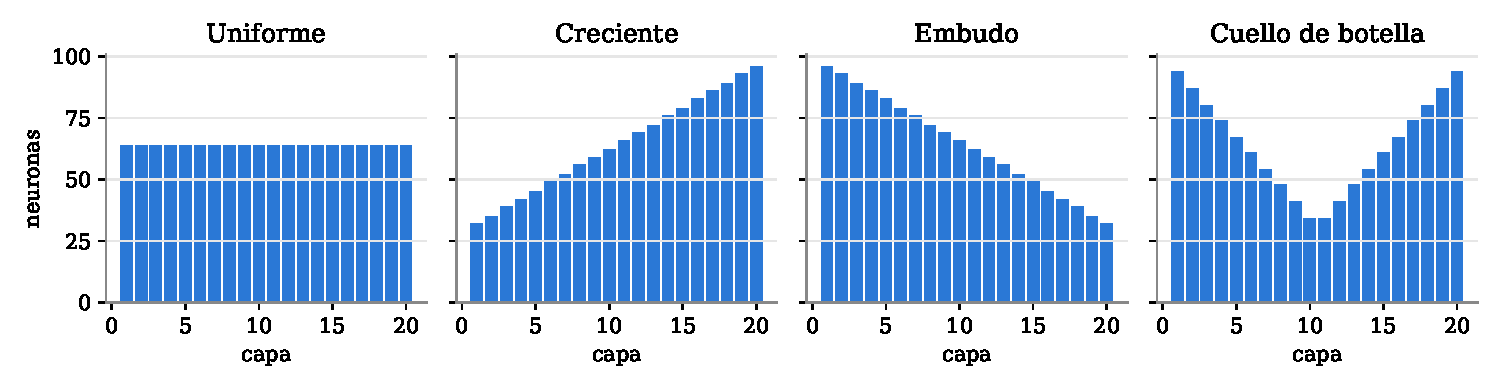
\includegraphics[width=\linewidth]{distribuciones.pdf}
\caption{Las cuatro formas con 20 capas y 1\,280 neuronas, calculadas con la función \code{distribuir\_neuronas} del notebook. Por ejemplo, el cuello de botella va de 94 neuronas en los extremos a 34 en el centro.}\label{fig:formas}
\end{figure}

\begin{proyecto}
Ganó la uniforme (AP 0.2721), seguida del embudo (0.2636), el cuello de botella (0.2619) y la creciente (0.2437).
\end{proyecto}

% =====================================================================
\needspace{8\baselineskip}
\section{Regularización y control del sobreajuste}

\subsection{Diagnóstico con curvas de aprendizaje}

Comparar las curvas de entrenamiento y validación es la herramienta básica de diagnóstico (Figura~\ref{fig:regimenes}):
\begin{itemize}
\item \textbf{Subajuste}: ambas pérdidas altas y planas; el modelo es demasiado simple o no aprende.
\item \textbf{Buen ajuste}: ambas bajan y se estabilizan juntas.
\item \textbf{Sobreajuste}: la de entrenamiento sigue bajando y la de validación sube; el modelo memoriza. La \textbf{brecha} entre ambas mide cuánto.
\end{itemize}

\begin{figure}[H]
\centering
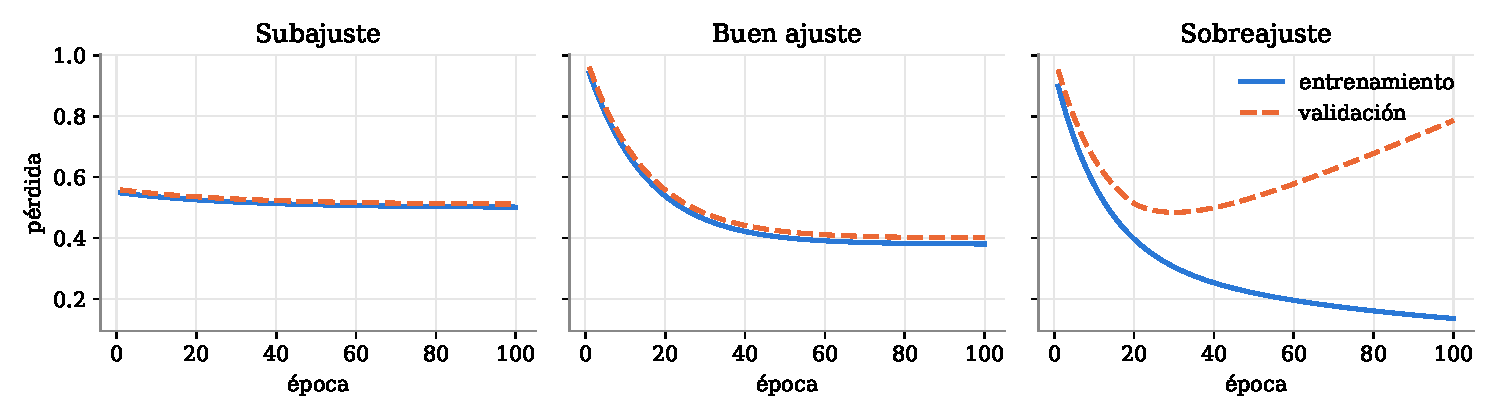
\includegraphics[width=\linewidth]{curvas_regimenes.pdf}
\caption{Curvas esquemáticas de los tres regímenes.}\label{fig:regimenes}
\end{figure}

\begin{proyecto}
En la corrida anterior, la red se entrenó 500 épocas sin control y se sobreajustó: AUC de 0.996 en entrenamiento y 0.582 en prueba. La red final tuvo 0.683 y 0.675.
\end{proyecto}

\subsection{\textit{Dropout}}

En cada paso de entrenamiento se apaga al azar una fracción $p$ de las neuronas de una capa (Srivastava et al., 2014). Así, la red no puede depender de una neurona concreta y aprende representaciones redundantes; equivale a promediar muchas subredes. En inferencia no se apaga nada. Keras usa \textit{inverted dropout}: durante el entrenamiento escala las neuronas activas por $1/(1-p)$ para que la salida esperada no cambie.

\begin{ejemplo}[: dropout con $p=0.25$]
Una capa con salidas $(0.8, 0.4, 1.2, 0.6)$ y máscara $(1,0,1,1)$ queda en $(0.8,0,1.2,0.6)/0.75=(1.067,0,1.6,0.8)$. En promedio se conserva la escala de la salida.
\end{ejemplo}

\begin{proyecto}
En la red de 20 capas, \textit{dropout} 0.25 bajó el AP de 0.2721 a 0.2520 y 0.50 hizo colapsar la red (AUC 0.543). Con pocos datos y una red ya limitada, apagar neuronas le quitó capacidad útil.
\end{proyecto}

\subsection{Regularización L1 y L2}

Se agrega a la pérdida una penalización sobre el tamaño de los pesos (Goodfellow et al., 2016):
\begin{equation}
\mathcal{L}_{\text{L1}} = \mathcal{L} + \lambda\sum_j|w_j|, \qquad
\mathcal{L}_{\text{L2}} = \mathcal{L} + \lambda\sum_j w_j^2 .
\end{equation}
La penalización L2 empuja cada peso con una fuerza proporcional a su tamaño ($2\lambda w$), así que achica los pesos sin anularlos. La L1 empuja con fuerza constante ($\lambda\,\text{signo}(w)$), así que lleva a cero los pesos pequeños y produce modelos dispersos, una forma implícita de selección de variables.

\begin{ejemplo}[: L1 frente a L2]
Con pesos $w=(0.5,\,-0.1)$ y $\lambda=10^{-4}$: la penalización L1 es $10^{-4}(0.5+0.1)=6\times10^{-5}$ y la L2 es $10^{-4}(0.25+0.01)=2.6\times10^{-5}$. El empuje L2 sobre el peso pequeño es $2\lambda(0.1)=2\times10^{-5}$, y el L1 es $10^{-4}$, cinco veces mayor. Por eso L1 anula antes los pesos pequeños.
\end{ejemplo}

\begin{proyecto}
L1 con $\lambda=10^{-4}$ recuperó parte de lo que había perdido el \textit{dropout}: el AP subió de 0.2520 a 0.2640, frente a 0.2586 con L2.
\end{proyecto}

\subsection{\textit{Early stopping} y paciencia}\label{sec:es}

Se vigila una métrica de validación y se detiene el entrenamiento cuando no mejora durante \textbf{paciencia} épocas seguidas; con \code{restore\_best\_weights=True} se recuperan los pesos de la mejor época (Prechelt, 1998). Decide automáticamente el número de épocas y frena el sobreajuste.

\begin{ejemplo}[: paciencia 5]
Si el AP de validación es máximo en la época 18 y no mejora en las épocas 19 a 23, el entrenamiento se detiene en la época 23 y se restauran los pesos de la época 18. Con paciencia 50, se habría seguido hasta la época 68 para terminar restaurando la misma época 18.
\end{ejemplo}

\begin{proyecto}
Las paciencias 5, 10, 20 y 50 dieron exactamente el mismo AP (0.2640), porque restauraron los mismos pesos; solo cambió el tiempo, de 89\,s a 251\,s.
\end{proyecto}

\begin{clave}
Las técnicas contra el sobreajuste (\textit{dropout}, L1/L2, \textit{early stopping}) solo ayudan si hay sobreajuste. Si el modelo ya generaliza bien, o está limitado por la información de los datos, pueden empeorarlo.
\end{clave}

% =====================================================================
\needspace{8\baselineskip}
\section{Modelos base}

\subsection{Regresión logística}

Modela el \textit{log-odds} de impago como una función lineal de las variables:
\begin{equation}
\ln\frac{p}{1-p} = \beta_0 + \sum_j \beta_j x_j, \qquad p=\frac{1}{1+e^{-(\beta_0+\sum_j\beta_jx_j)}} .
\end{equation}
Equivale a una red sin capas ocultas con salida sigmoide. Cada coeficiente se interpreta así: al aumentar $x_j$ en una unidad, las \textit{odds} se multiplican por $e^{\beta_j}$, con las demás variables fijas.

\begin{ejemplo}[: interpretar un coeficiente]
En el proyecto, el coeficiente de \code{int\_rate} es 1.773. Como la variable está escalada a $[0,1]$, pasar de la tasa mínima a la máxima multiplica las \textit{odds} de impago por $e^{1.773}=5.9$.
\end{ejemplo}

\subsection{Árbol de decisión}

Divide los datos con preguntas del tipo «¿\code{int\_rate} $>$ 0.4?» y elige en cada nodo la división que más reduce la \textbf{impureza de Gini}:
\begin{equation}
G = 1 - \sum_c p_c^2 .
\end{equation}

\begin{ejemplo}[: reducción de impureza]
Un nodo con 100 préstamos y 15 impagos tiene $G=1-(0.85^2+0.15^2)=0.255$. Una división lo separa en 60 préstamos con 3 impagos ($G=1-(0.95^2+0.05^2)=0.095$) y 40 con 12 impagos ($G=1-(0.7^2+0.3^2)=0.42$). La impureza ponderada queda en $0.6(0.095)+0.4(0.42)=0.225$, una reducción de $0.030$. La \textbf{importancia} de una variable es la suma de estas reducciones en todos los nodos donde se usa.
\end{ejemplo}

\subsection{\textit{Random Forest}}

Promedia muchos árboles, cada uno entrenado con una muestra \textit{bootstrap} de los datos y considerando en cada división solo un subconjunto aleatorio de variables. Promediar árboles poco correlacionados reduce la varianza sin aumentar mucho el sesgo.

\begin{proyecto}
Parámetros usados: árbol con profundidad máxima 5; \textit{Random Forest} con 150 árboles, 5 variables por división y 12 hojas como máximo. Ambos con y sin \code{class\_weight}. En prueba, la logística, el \textit{Random Forest} y las redes empataron (AUC de 0.675 a 0.677).
\end{proyecto}

% =====================================================================
\needspace{8\baselineskip}
\section{Interpretabilidad}

\subsection{Intrínseca frente a \textit{post hoc}}

Un modelo es \textbf{intrínsecamente interpretable} si su estructura se puede leer directamente, como los coeficientes de una logística o las reglas de un árbol pequeño. Los métodos \textbf{\textit{post hoc}} explican un modelo ya entrenado desde afuera, sin mirar su interior. Así se explica una red neuronal.

\subsection{SHAP}

SHAP reparte la salida de un préstamo entre sus variables usando valores de Shapley de la teoría de juegos (Lundberg \& Lee, 2017):
\begin{equation}
f(x) = \mathbb{E}[f(X)] + \sum_{j=1}^{M}\phi_j(x).
\end{equation}
Aquí $\mathbb{E}[f(X)]$ es la salida promedio sobre un conjunto de referencia (\textit{background}) y $\phi_j$ es lo que la variable $j$ sube o baja la salida en ese préstamo. Esta igualdad se llama \textbf{aditividad}. Para una red de clasificación se trabaja en \textit{log-odds}, donde la descomposición es aditiva, y se vuelve a probabilidad con $p=1/(1+e^{-f})$.

\begin{ejemplo}[: del SHAP a la probabilidad]
En el préstamo más riesgoso de la prueba, $\mathbb{E}[f(X)]=-1.851$, es decir, $p=1/(1+e^{1.851})=0.136$. Las contribuciones suman $+1.197$: \code{purpose\_small\_business} $+0.31$, \code{grade\_F} $+0.23$, \code{term} $+0.18$, y otras. La salida queda en $f(x)=-0.654$, que corresponde a $p=1/(1+e^{0.654})=0.342$.
Un SHAP de $+0.31$ significa $+0.31$ en \textit{log-odds}, no 31 puntos de probabilidad.
\end{ejemplo}

\textbf{Importancia global SHAP:} el promedio de $|\phi_j|$ sobre muchos préstamos. \textbf{Gráfico \textit{beeswarm}:} un punto por préstamo; el color indica el valor de la variable y la posición, su efecto.

\begin{clave}
Coeficientes, importancias de impureza y SHAP describen cómo \emph{el modelo} usa las variables, no relaciones causales. Si dos variables están correlacionadas (como la tasa y el grado), cada modelo puede repartir entre ellas el mismo efecto de forma distinta.
\end{clave}

% =====================================================================
\needspace{8\baselineskip}
\section{Tabla resumen de hiperparámetros}\label{sec:resumen}

\begin{table}[H]
\centering
\scriptsize
\renewcommand{\arraystretch}{1.25}
\begin{tabularx}{\linewidth}{>{\raggedright}p{2.1cm}>{\raggedright}p{3.1cm}XX>{\raggedright\arraybackslash}p{2.1cm}}
\toprule
Hiperparámetro & Qué controla & Si es muy bajo / poco & Si es muy alto / mucho & Valor elegido \\
\midrule
Optimizador & cómo se usa el gradiente & -- & -- & Adam \\
Tasa de aprendizaje & tamaño del paso & aprendizaje lento, se estanca & oscila o diverge & 0.0001 \\
Lote & gradiente por actualización & gradiente ruidoso, lento por época & menos actualizaciones, generaliza peor & 32 \\
Activación & no linealidad & -- & -- & tanh \\
Capas & profundidad & no capta relaciones complejas & desvanecimiento del gradiente, sobreajuste & 20 \\
Neuronas & ancho & poca capacidad & sobreajuste, costo & 64 \\
\textit{Dropout} & fracción apagada & sin efecto regularizador & pierde capacidad, colapsa & 0.25 \\
L1 / L2 ($\lambda$) & tamaño de los pesos & sin efecto & pesos casi nulos, subajuste & L1, $10^{-4}$ \\
Paciencia & tolerancia antes de parar & se detiene por ruido & gasta tiempo, o sobreajusta sin restaurar & 5 \\
Épocas & pasadas por los datos & subajuste & sobreajuste si no hay parada & 50 \\
Pesos de clase & costo de cada error & ignora la clase rara con $t=0.5$ & sobredetecta (resuelto igual con el umbral) & sin pesos \\
\bottomrule
\end{tabularx}
\caption{Resumen de hiperparámetros, efectos típicos y valores elegidos en la red mejorada del proyecto.}
\end{table}

% =====================================================================
\needspace{8\baselineskip}
\section{Preguntas de repaso}\label{sec:preguntas}

\begin{enumerate}[label=\textbf{\arabic*.}, leftmargin=*]
\item \textbf{Un modelo tiene 85\,\% de exactitud y F1 = 0. ¿Qué está pasando?}\\
Predice siempre la clase mayoritaria. Con 85\,\% de préstamos pagados, decir siempre «pagado» da esa exactitud sin detectar ningún impago.

\item \textbf{¿Por qué AP y AUC no cambian al mover el umbral?}\\
Porque dependen solo del orden de las probabilidades, y el umbral no cambia ese orden.

\item \textbf{¿Cuál es el AP de un modelo aleatorio en este problema?}\\
La prevalencia de impago, 0.148. El AUC de un modelo aleatorio es 0.5.

\item \textbf{¿Por qué los pesos de clase no mejoraron el AP?}\\
Porque desplazan todas las probabilidades por casi la misma cantidad en \textit{log-odds}: cambian el F1 con $t=0.5$, pero no el orden de los préstamos.

\item \textbf{¿Qué ventaja y qué desventaja tiene la búsqueda secuencial?}\\
Ventaja: su costo es la suma, no el producto, de los valores probados. Desventaja: ignora interacciones y depende del orden de las etapas.

\item \textbf{¿Por qué conviene incluir el valor vigente en cada etapa?}\\
Para que la etapa pueda conservarlo si ninguna alternativa mejora. En el proyecto, sin la opción de 0 en la etapa de \textit{dropout}, el AP bajó de 0.2721 a 0.2520.

\item \textbf{¿Por qué una red de 100 capas puede quedar en AUC $\approx$ 0.5?}\\
Por el desvanecimiento del gradiente: el producto de muchas derivadas menores que 1 deja las primeras capas sin aprender.

\item \textbf{¿En qué se diferencian L1 y L2?}\\
L2 achica los pesos en proporción a su tamaño. L1 empuja con fuerza constante y lleva a cero los pesos pequeños (selección de variables).

\item \textbf{¿Por qué todas las paciencias dieron el mismo resultado?}\\
Porque todas restauraron los pesos de la misma mejor época; una paciencia mayor solo añadió épocas de espera.

\item \textbf{Si dos modelos muy distintos llegan al mismo AUC, ¿qué sugiere?}\\
Que el límite está en la información de las variables y no en el modelo. Para mejorar, hay que construir mejores variables.

\item \textbf{¿Qué significa un SHAP de $+0.31$ en \textit{log-odds}?}\\
Que esa variable sube la salida en 0.31 \textit{log-odds}. El cambio en probabilidad depende del punto de partida; no son 31 puntos porcentuales.

\item \textbf{Calcula el F1 con VP = 40, FP = 60 y FN = 60.}\\
Precisión $=40/100=0.4$; \textit{recall} $=40/100=0.4$; F1 $=0.4$.
\end{enumerate}

% =====================================================================
\section*{Referencias}
\addcontentsline{toc}{section}{Referencias}
\begingroup
\setlength{\parindent}{-1cm}\setlength{\leftskip}{1cm}\setlength{\parskip}{4pt}\small

Bergstra, J., \& Bengio, Y. (2012). Random search for hyper-parameter optimization. \textit{Journal of Machine Learning Research, 13}, 281--305.

Glorot, X., \& Bengio, Y. (2010). Understanding the difficulty of training deep feedforward neural networks. En \textit{Proceedings of the Thirteenth International Conference on Artificial Intelligence and Statistics} (pp.~249--256). PMLR.

Goodfellow, I., Bengio, Y., \& Courville, A. (2016). \textit{Deep learning}. MIT Press.

Kingma, D. P., \& Ba, J. (2015). Adam: A method for stochastic optimization. En \textit{3rd International Conference on Learning Representations (ICLR)}.

Lundberg, S. M., \& Lee, S.-I. (2017). A unified approach to interpreting model predictions. En \textit{Advances in Neural Information Processing Systems 30} (pp.~4765--4774).

Prechelt, L. (1998). Early stopping---but when? En G. B. Orr \& K.-R. Müller (Eds.), \textit{Neural networks: Tricks of the trade} (pp.~55--69). Springer.

Saito, T., \& Rehmsmeier, M. (2015). The precision-recall plot is more informative than the ROC plot when evaluating binary classifiers on imbalanced datasets. \textit{PLoS ONE, 10}(3), e0118432.

Srivastava, N., Hinton, G., Krizhevsky, A., Sutskever, I., \& Salakhutdinov, R. (2014). Dropout: A simple way to prevent neural networks from overfitting. \textit{Journal of Machine Learning Research, 15}, 1929--1958.
\par\endgroup

\end{document}
